\documentclass{article}

\usepackage[francais]{babel}
\def\printlandscape{\special{landscape}}    % Works with dvips.
%\usepackage{pstricks,pst-node,pst-tree}
%\usepackage{amssymb}
\usepackage[utf8]{inputenc}
\usepackage[T1]{fontenc} 
\usepackage{fancybox} % for shadow and Bitemize
\usepackage{alltt}
\usepackage{graphicx}
\usepackage{caption} 

\usepackage{fancyvrb}
\usepackage{xcolor}

\definecolor{Zgris}{rgb}{0.87,0.85,0.85}

\newsavebox{\BBbox}
\newenvironment{DDbox}[1]{
\begin{lrbox}{\BBbox}\begin{minipage}{\linewidth}}
{\end{minipage}\end{lrbox}\noindent\colorbox{Zgris}{\usebox{\BBbox}} \\
[.5cm]}


%\usepackage{epsfig}
\usepackage{fullpage}
%\usepackage{fancyhdr}
%\usepackage{moreverb}
%\usepackage{xspace}
\usepackage[colorlinks,hyperindex,bookmarks,linkcolor=blue,citecolor=blue,urlcolor=blue]{hyperref}
\usepackage{array,multirow,makecell}
\setcellgapes{1pt}
\makegapedcells
\newcolumntype{R}[1]{>{\raggedleft\arraybackslash }b{#1}}
\newcolumntype{L}[1]{>{\raggedright\arraybackslash }b{#1}}
\newcolumntype{C}[1]{>{\centering\arraybackslash }b{#1}}
\usepackage{wrapfig}
\usepackage{epsf}

\title{Rapport de Projet GMIN332 :\\ Gestion de données complexes}

\author{Par : ALIJATE Mehdi - COUSOT Kevin - NEGROS Hadrien}

\date{15 Janvier 2014}

         
\begin{document}

\maketitle
\tableofcontents

\begin{abstract}
Accès et consultation de données provenant de différentes solutions de persistance (gros volumes de données distribuées et hétérogènes) au travers d'un démonstrateur.
\end{abstract}








\newpage 
%-----------------------------------------------------------
\section{Introduction}\label{sec:intro}
Les systèmes NoSQL et les technologies du Web Sémantique sont une altérnative aux SGBD classiques. Cependant, elles sont encore très loin d'être couramment utilisées, comme celles du monde relationnel "classique". \\
Néanmoins, de grands acteurs d'internet (\textit{comme Facebook (Cassandra Project puis HBase), Google (BigTable), Ubuntu One (CouchDB)... etc.}) commencent à exploiter des bases de données de type NoSQL. L'avantage de celà, c'est que la majorité de ces projets est open source et sous licence libre.
\\
Dans notre projet, nous avons voulu explorer les différentes technologies qui puissent gérer des données RDF. Nous avons donc étudié une solution basée sur le mapping de bases relationnelles (\textbf{D2RQ}), et des solutions basées sur des bases NoSQL (\textbf{TDB, Hbase et Neo4j}).
\\
Le but de ce projet est d’exploiter différentes sources de données, gérées au travers de plusieurs systèmes de gestion de données, afin de permettre un accès et consultation de ces derniers. Ceci, via une application permettant d'interconnecter ces sources de données, basée sur l'API de Jena.





%-----------------------------------------------------------

\section{Jeu de données}

\subsection{Description}
Le jeu de données utilisé représente des données de vocabulaire de l'\textbf{INSEE} et des données\textbf{ Geonames}.
L’INSEE (Institut National de la Statistique et des Etudes Economiques) collecte, produit, analyse et diffuse des informations sur l'économie et la société françaises. A ce titre, il conduit des recensements et des enquêtes, il gère des bases de données et exploite aussi des sources administratives.
Geonames est une base de données géographique gratuite et librement accessible sur Internet (www.geonames.org). La base regroupe plus de 8 millions de noms de lieux géographiques, et beaucoup d’informations autours de ces lieux (par exemple la  population, la subdivision administrative, le code postal, la latitude, la longitude, l'altitude, etc.). 
\\
\subsection{Schéma}


\textbf{//A finir avec une description plus précise de chaque données avec un schéma d'interconnexion
}

\section{Analyse du système}

\subsection{Différents modèles de représentation des données}

\subsubsection{Modèle relationnel}
Le modèle relationnel est le modèle de représentation le plus utilisé dans les SGBD actuellement. Il est basé sur l'algèbre relationnelle. Une BDD relationnelle est un ensemble de \textit{tuples} groupés ensemble dans des \textit{tables}, et un ensemble de contraintes qui, entre autre, permettent de définir des liens entre les tables.
Pour pouvoir exploiter des données stockées dans une BDD relationelle en meme temps que des données stockée dans des BDD NoSQL, nous avons besoin d'une interface qui nous permettra de requêter dans un langage commun, différent donc de SQL.\\
Le SGBD que nous avons choisi est \textbf{MySQL}, et l'interface \textbf{D2RQ}.
\subsubsection{Triple Store}
Un Triple Store est une base de donnée NoSQL conçue pour stocker des triplets RDFs. La consultation des données se fait avec le langage de requête \textbf{Sparql}. 
La création d'un TDB store à pour effet de creer des fichiers persistant dans un dossier précisé en entrée. Les fichiers de données RDF sont donc chargés une fois, puis l'accès aux données se fait en chargeant ce dossier dans notre application. Le seul type de donnée qu'un triple store peut stocker est le \textit{triplet}. Contrairement au relationnel, ce modèle ne dépend donc pas d'un schéma.\\
Le triple store que nous avons décidé d'intégrer est \textbf{TDB}.
\subsubsection{Base de données orientée graphe}
Une base de données orientée graphe est une BDD NoSQL utilisant la théorie des graphes. Les données sont donc représentées sous forme de noeuds et d'arcs représentant ces noeuds. Ce modèle est pratique pour la représentation de données, car dans beaucoup de cas les données sont facilement représentables sous forme de graphe.\\
La base de donnée orientée graphe que nous avons décidé d'intégré est \textbf{Neo4j}
\subsubsection{Base de données orientée colonnes}\label{sec:Hbase}
Une base de données orientée colonne est une BDD qui stocke les données sous forme de colonnes, contrairement aux BDD relationnelles qui les stockent par lignes (tuples). \\
L'intérêt est de sérialisé les colonnes les unes après les autres, alors que l'orientation "ligne" écrit chaque entité les unes après les autres.\\
Les lignes des tables sont partitionnées en plusieurs regions, qui sont stockées dans des region servers. Celles-ci se créent automatiquement au fûr et à mesur de l'augmentation de la taille (un seuil limite est défini). Ainsi, le contenu des region servers est indexé dans un serveur master, qui dirge les clients vers le nœud adéquat. \\
Enfin, ZooKeeper est un logiciel de gestion de configuration pour systèmes distribués. Celui-ci est utilisé pour définir les instances Hadoop faisant partie du cluster HBase. Le fonctionnement de Hbase est expliqué dans le schéma suivant : 
\begin{center}
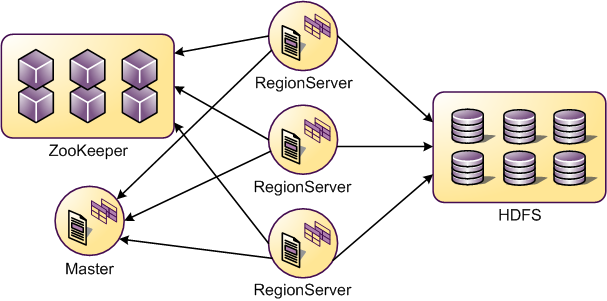
\includegraphics[scale=0.5]{hbase-shema.png} 
\captionof{figure}{Vue Générale du fonctionnement de Hbase}
\label{fig_hbase}
\end{center}
Source :  Cf. Hbase dans \ref{sec:shbase}.


 
\subsection{Une API pour les gouverner tous: Jena}\label{sec:Jena}

Jena est une API Java qui peut être utilisée pour créer et manipuler des données RDF . Jena possède des classes pour représenter des graphes, des ressources, des propriétés et des littéraux.

Ce projet est uni autour de l'API de Jena (Cf. Section \ref{sec:Jena}) et de ses modèles.
\begin{center}
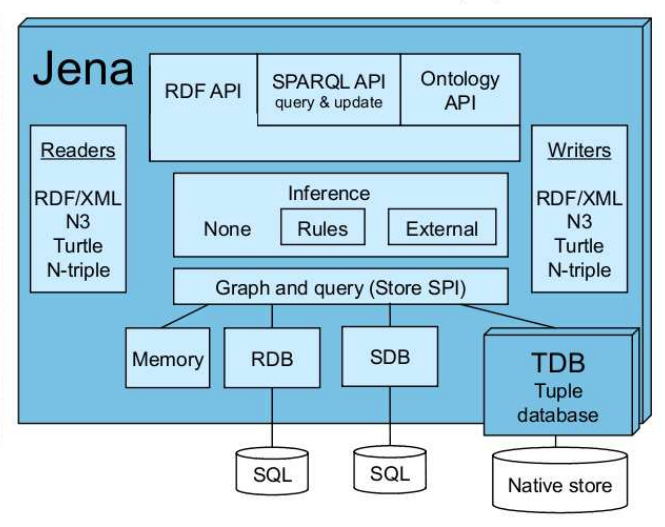
\includegraphics[scale=0.5]{archi_jena.jpeg} 
\captionof{figure}{Vue Générale de l'architecture JENA}
\label{fig_jena}
\end{center}

\begin{center}
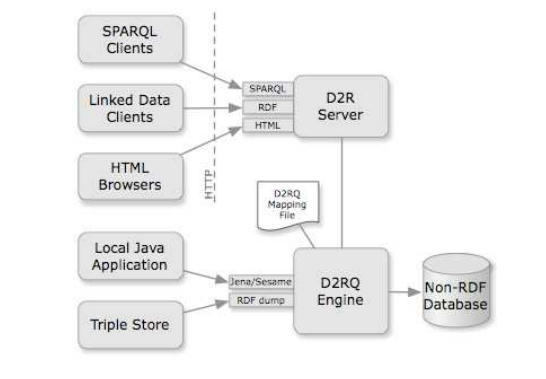
\includegraphics[scale=0.5]{archi_D2RQ.jpeg} 
\captionof{figure}{Vue Générale de l'architecture D2RQ}
\label{fig_d2rq}
\end{center}


\subsection{Le langage de requete SPARQL}\label{sec:Sparql}
La réprésentation Model spécifique à Jena a permis l'union obtenue à partir de nos sources de données. Les requêtes SPARQL sont effectuées sur le modèle ainsi créé.\\
Chaque triple store définit ses propres fonctions à côté de celles de SPARQL (ARQ pour Jena). Pour gérer les requêtes SPARQL, Jena utilise sa propre librairie \textit{ARQ}. Cette librairie définit également sa propre syntaxe, compatible notre mode de requêtage SPARQL, cela y ajoute des fonctionnalités semblables à ce qu'on peut trouver dans MySql par exemple, comme COUNT, MAX, etc, car ces fonctions ne sont pas gérées par défaut par SPARQL.



%-----------------------------------------------------------
\section{Application}
\subsection{Généralités}
Notre application se base sur un modèle JENA (Cf. \ref{sec:Jena}) construit, avec des données réparties, comme vu au dessus, au sein de différents systèmes de stockage\\
Le modèle JENA sert donc d'union ou interconnexion de ces données, pour qu'on puisse à la fin intérroger ce dernier via des requêtes SPARQL(Cf. \ref{sec:Sparql}), sur n'importe quel type de données sans devoir dépendre d'un type de stockage précis. 

\subsection{Architecture}
Le but est de pouvoir respecter l'architecture ou le schéma suivant : \\
\begin{center}
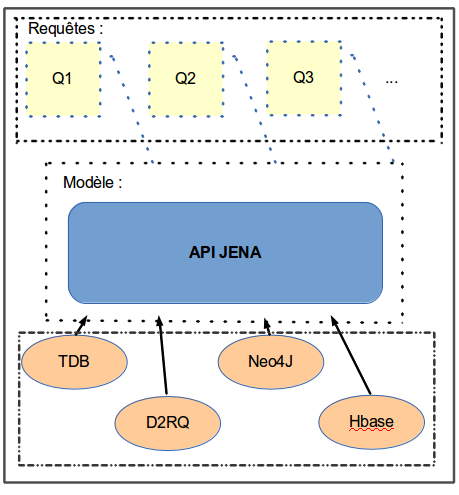
\includegraphics[scale=0.5]{archi_appli.png} 
\captionof{figure}{Architecture ou schéma de fonctionnement de l'application}
\label{fig_appli}
\end{center}
La génération du modèle se fait dans les classes correspondantes à nos systèmes, puisqu'une fonction pour chacun d'entre eux génère le mapping :
\begin{itemize}
\item Pour D2RQ : c'est la fonction //TODOOO avec une desc et screenshot de la fction
\item Pour TDB : //TODO Pareil
\item Pour Ne4j : la fonction //TODO construit unmodèle jena à partir d'une bdd embarquée neo4j. //Manque screenshot
\end{itemize}
Une fois le modèle JENA construit, l'union y est faite, facilitant l'interrogation de ce modèle.


\section{Démonstration}

\subsection{Principe}
//TODO

\subsection{Requêtes}

Donner l'ensemble des résidences de tourismes avec leurs codes postales dans le Calvados (14) : \\

\begin{DDbox}{\linewidth}
\begin{Verbatim}
        float cosinus  (float x, int maxIteration)
        {
           /* encore du code ici */
        }
\end{Verbatim}
\end{DDbox}
%-----------------------------------------------------------


\section{Discussion et Conclusion }
Durant la réalisation de ce projet, il a été constaté qu'il serait plus intéréssant de distribuer les donéees sur des sites différents et notamment, pour Neo4j, ne pas utiliser une bdd embarquée mais l'api REST. C'est l'une des perspectives pour la complétion de ce travail dans le futur.\\

Mais l'une des difficultés majeures rencontrer c'est celle concernant l'installation et l'exploitation de la base de données orientée colonnes : Hbase, Cf. \ref{sec:Hbase}.\\
En effet, le choix du type de base de donnée NoSQL (en l'occurence dans ce cas là, celle orientée colonnes) et la manière de stocker les données en structurant les triples pour celle-ci,  afin de la lier avec les autres via l'API JENA ne relève pas de l'impossible, mais reste très difficile, ceci est dû principalement au manque de documentations.\\
Malgré les difficultés rencontrées pour la mise en place de ce système d'interconnexion des sources de données, ce projet nous a avant tout permis de se familiariser et d'expérimenter l'API Jena, en complément au processus théorique et expérimental vu en Cours et TP durant le semestre.\\
Nous avons en fin de compte pu intégrer 3 solutions sur les 4 initiales (D2RQ, TDB et Neo4j), et nous avons pu intérroger le modèle faisant office de l'union de ces derniers.\\
On peut dire qu'on a retenu que l'interconnexion des données simplifie énormement l'exploitation de celle-ci, puisque le système voulant les exploiter devient plus performant ainsi.
%-----------------------------------------------------------


\section{Sources}
\begin{itemize}
\item API Jena et TDB : \href{http://jena.apache.org/}{http://jena.apache.org/}
 \\
\item D2RQ : \href{http://d2rq.org/}{http://d2rq.org/}
\\
\item Neo4J : \href{http://neo4j.org/}{http://neo4j.org/}
\\
\item Hbase :\label{sec:shbase}
\begin{itemize}
\item \href{http://blog.xebia.fr/2009/11/18/devoxx-jour-1-nosql-avec-hbase/}{http://blog.xebia.fr/2009/11/18/devoxx-jour-1-nosql-avec-hbase/}
 \item \href{http://hbase.apache.org/}{http://hbase.apache.org/}
\end{itemize}

\item SPARQL : \href{http://www.sparql.org/}{http://www.sparql.org/}
\\
\item Geonames : \href{http://www.geonames.org/}{http://www.geonames.org/}
\\
\item INSEE : \href{http://rdf.insee.fr/}{http://rdf.insee.fr/}
\\
\item Données sur le tourisme : \href{http://data.gouv.fr/fr/dataset/residences-de-tourisme-classees-en-france/}{http://data.gouv.fr/fr/dataset/residences-de-tourisme-classees-en-france/}

\end{itemize}

%-----------------------------------------------------------

\end{document}

%%% Local Variables:
%%% mode: latex
%%% TeX-master: t
%%% coding: utf-8
%%% End:
